\documentclass[aspectratio=169]{beamer}
\usepackage[latin1]{inputenc}
\usepackage{tikz}
\usetikzlibrary{calc}
\usetikzlibrary{arrows}
\usetheme{Warsaw}
\setbeamertemplate{navigation symbols}{}
\title[Whats this]{No need}
\author{Luke}
\institute{Somewhere}
\date{Today}

\begin{document}

\begin{frame}[plain]{}
  \begin{exampleblock}{}
    {\LARGE Considerations for TAO}
  \end{exampleblock}
  \Large
  \begin{itemize}
    \item Must handle large datasets.
    \item Average request in hours (ideally minutes).
    \item Scale over large number of distributed cores.
    \item Use an SQL capable DB.
  \end{itemize}
  \begin{columns}[c]
    \column{3cm}
    \column{4cm}
    \begin{exampleblock}{}
      How to choose a DBMS?
    \end{exampleblock}
  \end{columns}
\end{frame}

\begin{frame}[plain]
    \hspace{2cm}
    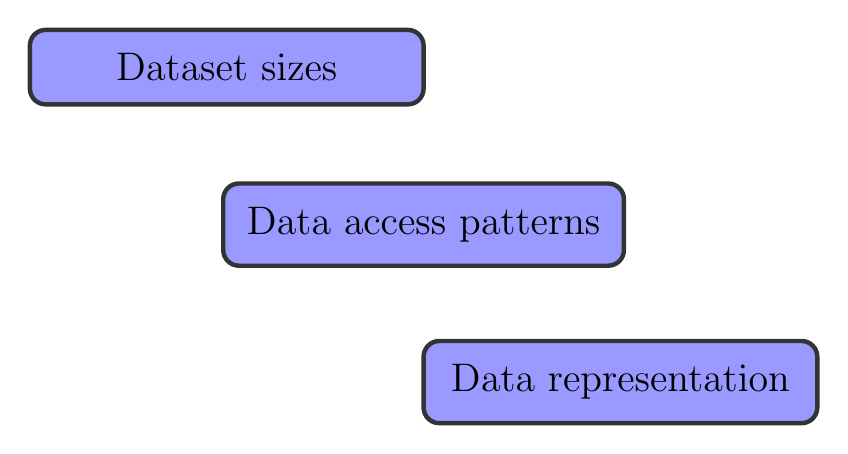
\begin{tikzpicture}[
        norm/.style={draw=black!80,rectangle,rounded corners=2mm,inner sep=3mm,fill=blue!40,ultra thick,minimum width=5cm},
        lit/.style={draw=black!80,rectangle,rounded corners=2mm,inner sep=3mm,fill=red!80,ultra thick,minimum width=5cm}
      ]
      \node[norm] at (0,-0) {{\Large Dataset sizes}};
      \node[norm] at (2.5,-2) {{\Large Data access patterns}};
      \node[norm] at (5,-4) {{\Large Data representation}};
    \end{tikzpicture}
\end{frame}

\begin{frame}[plain]
    \hspace{2cm}
    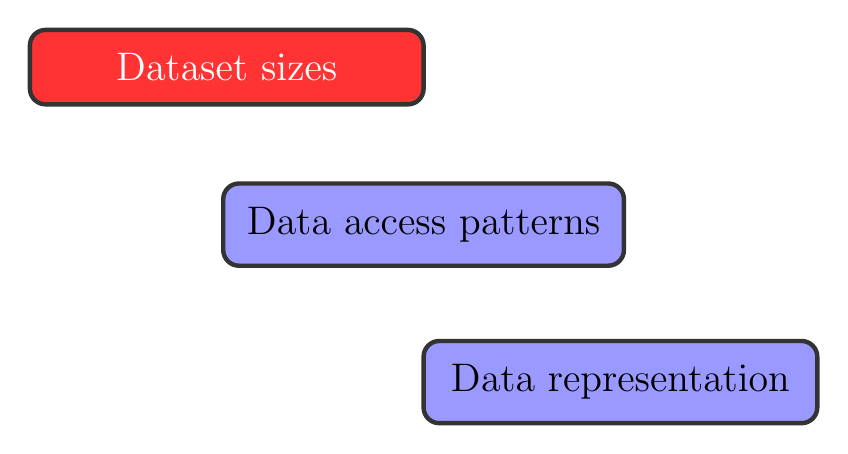
\begin{tikzpicture}[
        norm/.style={draw=black!80,rectangle,rounded corners=2mm,inner sep=3mm,fill=blue!40,ultra thick,minimum width=5cm},
        lit/.style={draw=black!80,rectangle,rounded corners=2mm,inner sep=3mm,fill=red!80,ultra thick,minimum width=5cm}
      ]
      \node[lit] at (0,0) {{\Large \textcolor{white}{Dataset sizes}}};
      \node[norm] at (2.5,-2) {{\Large Data access patterns}};
      \node[norm] at (5,-4) {{\Large Data representation}};
    \end{tikzpicture}
\end{frame}

\begin{frame}[plain]
  \begin{block}{Millennium}
    \begin{itemize}
    \item $\approx$ 750,000,000 galaxies
    \item $\approx$ 300GB
    \item \url{http://www.mpa-garching.mpg.de/galform/virgo/millennium}
    \end{itemize}
  \end{block}
  \begin{block}{Bolshoi}
    \begin{itemize}
    \item $\approx$ 2,500,000,000 galaxies
    \item $\approx$ 1TB
    \item \url{http://hipacc.ucsc.edu/Bolshoi}
    \end{itemize}
  \end{block}
\end{frame}

\begin{frame}[plain]
    \hspace{2cm}
    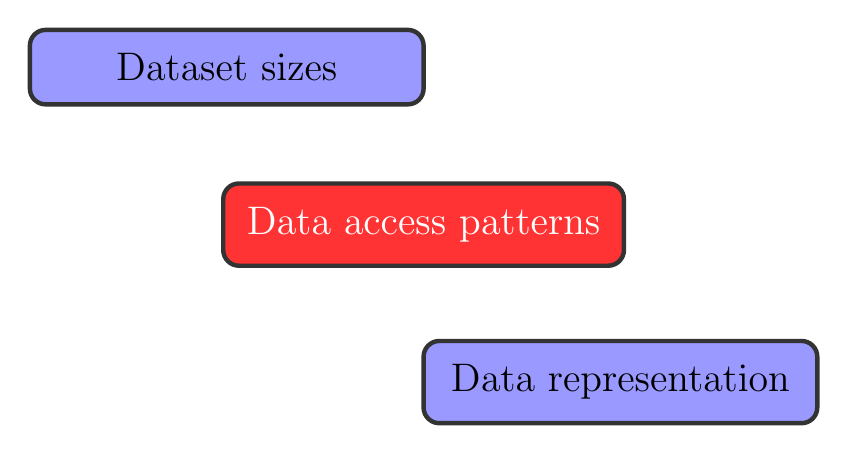
\begin{tikzpicture}[
        norm/.style={draw=black!80,rectangle,rounded corners=2mm,inner sep=3mm,fill=blue!40,ultra thick,minimum width=5cm},
        lit/.style={draw=black!80,rectangle,rounded corners=2mm,inner sep=3mm,fill=red!80,ultra thick,minimum width=5cm}
      ]
      \node[norm] at (0,0) {{\Large Dataset sizes}};
      \node[lit] at (2.5,-2) {{\Large \textcolor{white}{Data access patterns}}};
      \node[norm] at (5,-4) {{\Large Data representation}};
    \end{tikzpicture}
\end{frame}

\begin{frame}[plain]
  \begin{block}{Science Modules}
    \vspace{1cm}
    \hspace{2cm}
    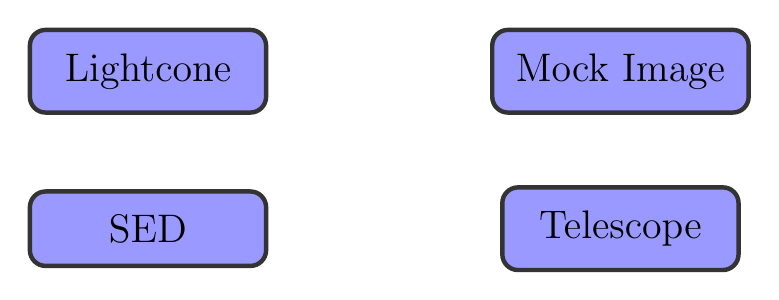
\begin{tikzpicture}[
        norm/.style={draw=black!80,rectangle,rounded corners=2mm,inner sep=3mm,fill=blue!40,ultra thick,minimum width=3cm}
      ]
      \node[norm] at (0,0) {{\Large Lightcone}};
      \node[norm] at (0,-2) {{\Large SED}};
      \node[norm] at (6,0) {{\Large Mock Image}};
      \node[norm] at (6,-2) {{\Large Telescope}};
    \end{tikzpicture}
    \vspace{1cm}
  \end{block}
\end{frame}

\begin{frame}[plain]
  \begin{block}{Science Modules}
    \vspace{1cm}
    \hspace{2cm}
    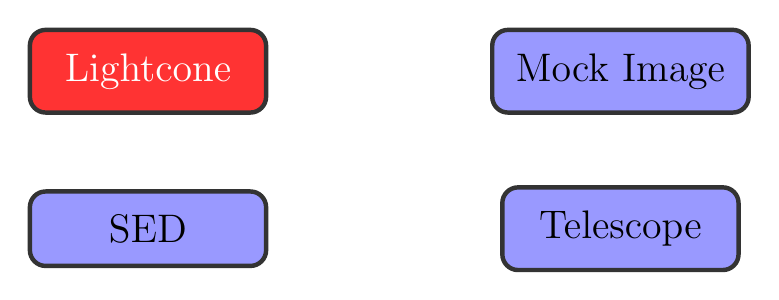
\begin{tikzpicture}[
        norm/.style={draw=black!80,rectangle,rounded corners=2mm,inner sep=3mm,fill=blue!40,ultra thick,minimum width=3cm},
        lit/.style={draw=black!80,rectangle,rounded corners=2mm,inner sep=3mm,fill=red!80,ultra thick,minimum width=3cm}
      ]
      \node[lit] at (0,0) {{\Large \textcolor{white}{Lightcone}}};
      \node[norm] at (0,-2) {{\Large SED}};
      \node[norm] at (6,0) {{\Large Mock Image}};
      \node[norm] at (6,-2) {{\Large Telescope}};
    \end{tikzpicture}
    \vspace{1cm}
  \end{block}
\end{frame}

\begin{frame}[plain]
  \hspace{2cm}
  \begin{tikzpicture}
    \path[use as bounding box] (0,-1) rectangle (10,7);
    % Border.
    \draw (0,0) rectangle(6,6);
    
    \draw[-triangle 90] (8,5.5) node[anchor=west] {simulation domain} -- (6,5);
  \end{tikzpicture}
\end{frame}

\begin{frame}[plain]
  \hspace{2cm}
  \begin{tikzpicture}
    \path[use as bounding box] (0,-1) rectangle (10,7);
    % Border.
    \draw (0,0) rectangle(6,6);
    \draw[-triangle 90] (8,5.5) node[anchor=west] {simulation domain} -- (6,5);
    % Objects.
    \pgfmathsetseed{1187}
    \foreach \x in {1,...,100}
    \fill[black!50] ($ (0,0) + 6*(rnd,rnd) $) circle(1pt);
    \draw[-triangle 90] (8,4.5) node[anchor=west] {galaxies} -- (5,4);
  \end{tikzpicture}
\end{frame}

\begin{frame}[plain]
  \hspace{2cm}
  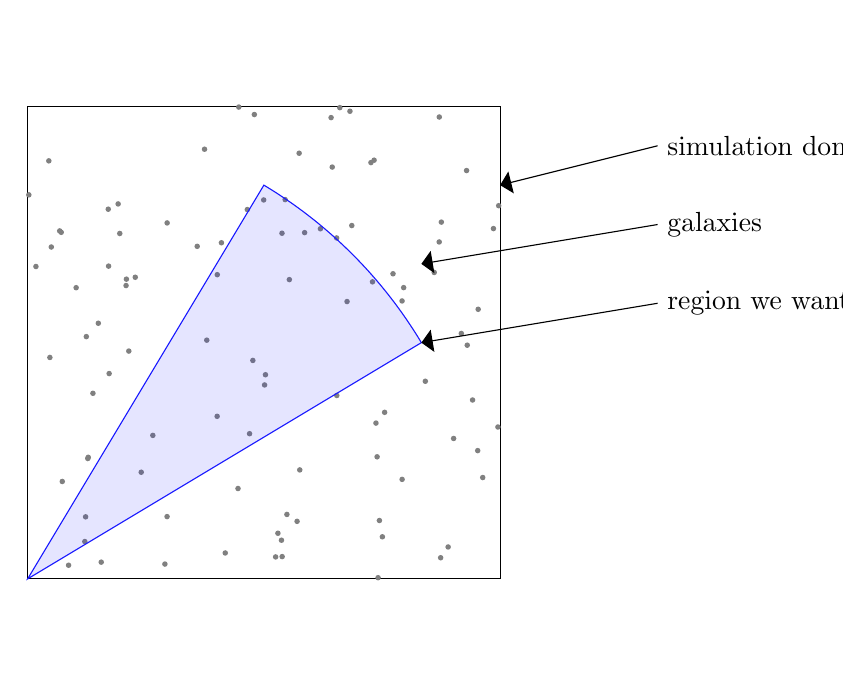
\begin{tikzpicture}
    \path[use as bounding box] (0,-1) rectangle (10,7);
    % Border.
    \draw (0,0) rectangle(6,6);
    \draw[-triangle 90] (8,5.5) node[anchor=west] {simulation domain} -- (6,5);
    % Objects.
    \pgfmathsetseed{1187}
    \foreach \x in {1,...,100}
    \fill[black!50] ($ (0,0) + 6*(rnd,rnd) $) circle(1pt);
    \draw[-triangle 90] (8,4.5) node[anchor=west] {galaxies} -- (5,4);
    % Cone.
    \filldraw[fill=blue,fill opacity=0.1,draw=blue!90] (0,0) -- (5,3) arc (30.96:59.04:5.83) -- cycle;
    \draw[-triangle 90] (8,3.5) node[anchor=west] {region we want} -- (5,3);
  \end{tikzpicture}
\end{frame}

\begin{frame}[plain]
  \hspace{2cm}
  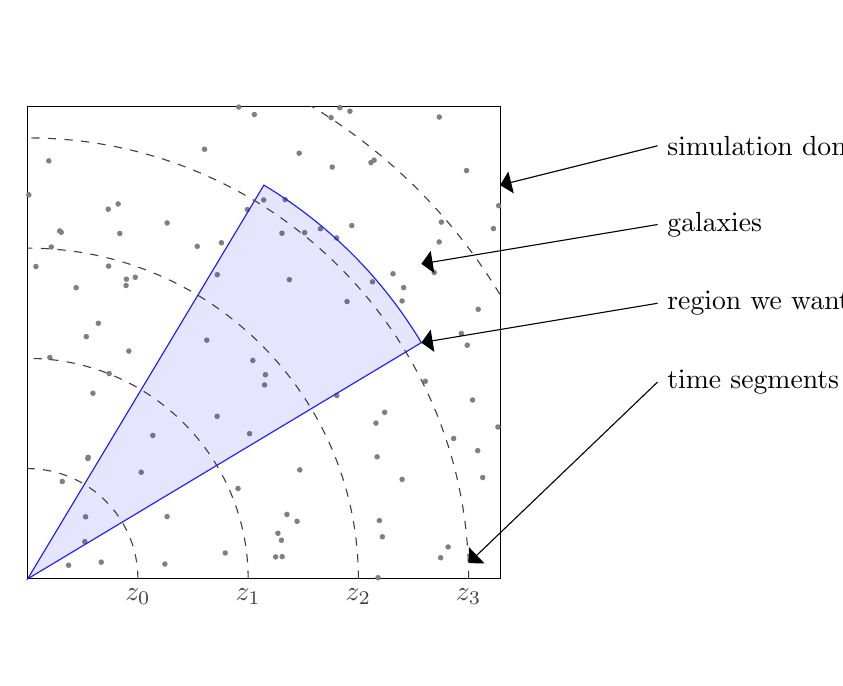
\begin{tikzpicture}
    \path[use as bounding box] (0,-1) rectangle (10,7);
    % Border.
    \draw (0,0) rectangle(6,6);
    \draw[-triangle 90] (8,5.5) node[anchor=west] {simulation domain} -- (6,5);
    % Objects.
    \pgfmathsetseed{1187}
    \foreach \x in {1,...,100}
    \fill[black!50] ($ (0,0) + 6*(rnd,rnd) $) circle(1pt);
    \draw[-triangle 90] (8,4.5) node[anchor=west] {galaxies} -- (5,4);
    % Cone.
    \filldraw[fill=blue,fill opacity=0.1,draw=blue!90] (0,0) -- (5,3) arc (30.96:59.04:5.83) -- cycle;
    \draw[-triangle 90] (8,3.5) node[anchor=west] {region we want} -- (5,3);
    % Redshift arcs.
    \begin{scope}
      \clip (0,-1) rectangle(6,6);
      \foreach \x/\z in {1.4/0, 2.8/1, 4.2/2, 5.6/3, 7/4}
        \draw[black!75,dashed] (\x,0) node[anchor=north]{$z_\z$} arc (0:90:\x);
    \end{scope}
    \draw[-triangle 90] (8,2.5) node[anchor=west] {time segments} -- (5.6,0.2);
  \end{tikzpicture}
\end{frame}

\begin{frame}[plain]
SELECT * FROM snapshot\_004 WHERE (9437.5 + IF(39.8397 + Pos1 $\langle$ 62.5, 39.8397 + Pos1, Pos1 + 39.8397-62.5) - 0) $\langle$ 9427.7048129608065 AND (9437.5 + IF(39.8397 + Pos1 $\langle$ 62.5, 39.8397 + Pos1, Pos1 + 39.8397-62.5) - 0) $\rangle$ 9408.2000081888491 AND (187.5 + IF(26.503 + Pos2 $\langle$ 62.5, 26.503 + Pos2, Pos2 + 26.503-62.5) - 3.45846e-323) $\langle$ 246.78854155076195 AND (187.5 + IF(26.503 + Pos2 $\langle$ 62.5, 26.503 + Pos2, Pos2 + 26.503-62.5) - 3.45846e-323) $\rangle$ 0 AND (187.5 + IF(55.9087 + Pos3 $\langle$ 62.5, 55.9087 + Pos3, Pos3 + 55.9087-62.5) - 6.90856e-310) $\langle$ 246.78854155076195 AND (187.5 + IF(55.9087 + Pos3 $\langle$ 62.5, 55.9087 + Pos3, Pos3 + 55.9087-62.5) - 6.90856e-310) $\rangle$ 0 AND SQRT(POW((9437.5 + IF(39.8397 + Pos1 $\langle$ 62.5, 39.8397 + Pos1, Pos1 + 39.8397-62.5) - 0), 2)
\end{frame}

\begin{frame}[plain]
+ POW((187.5 + IF(26.503 + Pos2 $\langle$ 62.5, 26.503 + Pos2, Pos2 + 26.503-62.5) - 3.45846e-323), 2) + POW((187.5 + IF(55.9087 + Pos3 $\langle$ 62.5, 55.9087 + Pos3, Pos3 + 55.9087-62.5) - 6.90856e-310), 2)) $\langle$ 9427.7048129608065 AND SQRT(POW((9437.5 + IF(39.8397 + Pos1 $\langle$ 62.5, 39.8397 + Pos1, Pos1 + 39.8397-62.5) - 0), 2) + POW((187.5 + IF(26.503 + Pos2 $\langle$ 62.5, 26.503 + Pos2, Pos2 + 26.503-62.5) - 3.45846e-323), 2) + POW((187.5 + IF(55.9087 + Pos3 $\langle$ 62.5, 55.9087 + Pos3, Pos3 + 55.9087-62.5) - 6.90856e-310), 2)) $\rangle$ 9414.6512343460909 AND SQRT(POW((9437.5 + IF(39.8397 + Pos1 $\langle$ 62.5, 39.8397 + Pos1, Pos1 + 39.8397-62.5) - 0), 2) + POW((187.5 + IF(26.503 + Pos2 $\langle$ 62.5, 26.503 + Pos2, Pos2 + 26.503-62.5) - 3.45846e-323), 2) + POW((187.5 + IF(55.9087 + Pos3 $\langle$ 62.5, 55.9087 + Pos3, Pos3 + 55.9087-62.5) - 6.90856e-310), 2)) $\langle$ 9427.7048129608065 AND
\end{frame}

\begin{frame}[plain]
(9437.5 + IF(39.8397 + Pos1 $\langle$ 62.5, 39.8397 + Pos1, Pos1 + 39.8397 - 62.5) - 0)/(SQRT(POW((9437.5 + IF(39.8397 + Pos1 $\langle$ 62.5, 39.8397 + Pos1, Pos1 + 39.8397 - 62.5) - 0), 2) + POW((187.5 + IF(26.503 + Pos2 $\langle$ 62.5, 26.503 + Pos2, Pos2 + 26.503 - 62.5) - 3.45846e-323), 2))) $\rangle$ 0.070737201667702906 AND (9437.5 + IF(39.8397 + Pos1 $\langle$ 62.5, 39.8397 + Pos1, Pos1 + 39.8397 - 62.5) - 0)/(SQRT(POW((9437.5 + IF(39.8397 + Pos1 $\langle$ 62.5, 39.8397 + Pos1, Pos1 + 39.8397 - 62.5) - 0), 2) + POW((187.5 + IF(26.503 + Pos2 $\langle$ 62.5, 26.503 + Pos2, Pos2 + 26.503-62.5) - 3.45846e-323), 2))) $\langle$ 1 AND SQRT(POW((9437.5 + IF(39.8397 + Pos1 $\langle$ 62.5, 39.8397 + Pos1, Pos1 + 39.8397-62.5) - 0), 2) + POW((187.5 + IF(26.503 + Pos2 $\langle$ 62.5, 26.503 + Pos2, Pos2 + 26.503-62.5) -
\end{frame}

\begin{frame}[plain]
3.45846e-323), 2))/(SQRT(POW((9437.5 + IF(39.8397 + Pos1 $\langle$ 62.5, 39.8397 + Pos1, Pos1 + 39.8397-62.5) - 0), 2) + POW((187.5 + IF(26.503 + Pos2 $\langle$ 62.5, 26.503 + Pos2, Pos2 + 26.503-62.5) - 3.45846e-323), 2) + POW((187.5 + IF(55.9087 + Pos3 $\langle$ 62.5, 55.9087 + Pos3, Pos3 + 55.9087-62.5) - 6.90856e-310), 2))) $\rangle$ 0.070737201667702906 AND SQRT(POW((9437.5 + IF(39.8397 + Pos1 $\langle$ 62.5, 39.8397 + Pos1, Pos1 + 39.8397-62.5) - 0), 2) + POW((187.5 + IF(26.503 + Pos2 $\langle$ 62.5, 26.503 + Pos2, Pos2 + 26.503-62.5) - 3.45846e-323), 2))/(SQRT(POW((9437.5 + IF(39.8397 + Pos1 $\langle$ 62.5, 39.8397 + Pos1, Pos1 + 39.8397-62.5) - 0), 2) + POW((187.5 + IF(26.503 + Pos2 $\langle$ 62.5, 26.503 + Pos2, Pos2 + 26.503-62.5) - 3.45846e-323), 2) + POW((187.5 + IF(55.9087 + Pos3 $\langle$ 62.5, 55.9087 + Pos3, Pos3 + 55.9087-62.5) - 6.90856e-310), 2))) $\langle$ 1
\end{frame}

\begin{frame}[plain]
  \hspace{2.5cm}{\Large Very large amount of data to search} \\
  \hspace{2cm}{\Large + Complicated SQL query} \\
  \hspace{2cm}{\Large + Multiple users} \\
  \hspace{2cm}{\Large = \alert{Trouble}}
  \vspace{1cm}
  \begin{alertblock}{Solution}
    \centering
    \vspace{0.5cm}
    {\Large Distribute over multiple servers.}
    \vspace{0.5cm}
  \end{alertblock}
\end{frame}

\begin{frame}[plain]
 \begin{block}{Distributed DBMS Systems}
 \begin{itemize}
   \item MySQL Cluster
     \begin{itemize}
       \item Difficult to manage.
     \end{itemize}
   \item pgpool
     \begin{itemize}
       \item Bugs with some queries.
     \end{itemize}
   \item PostgresXC
     \begin{itemize}
       \item Older PostgresQL.
       \item Small development team.
     \end{itemize}
   \item Custom (PostgresQL)
     \begin{itemize}
       \item Reinventing the wheel?
     \end{itemize}
 \end{itemize}
 \end{block}
\end{frame}

\begin{frame}[plain]
  \vspace{1cm}
  \begin{center}
 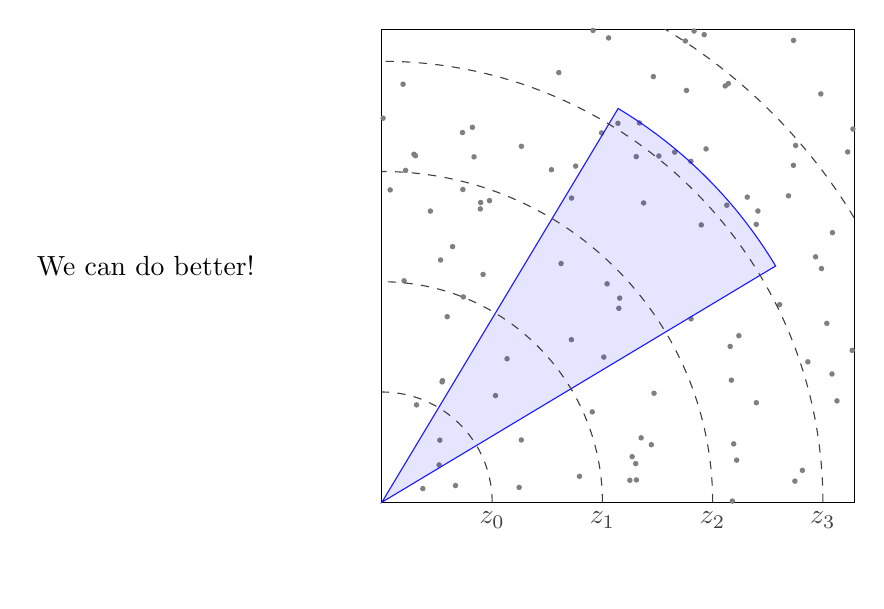
\begin{tikzpicture}
   % Text.
   \node at (-3,3) {We can do better!};
   % Border.
   \draw (0,0) rectangle(6,6);
   % Objects.
   \pgfmathsetseed{1187}
   \foreach \x in {1,...,100}
     \fill[black!50] ($ (0,0) + 6*(rnd,rnd) $) circle(1pt);
   % Cone.
   \filldraw[fill=blue,fill opacity=0.1,draw=blue!90] (0,0) -- (5,3) arc (30.96:59.04:5.83) -- cycle;
    % Redshift arcs.
    \begin{scope}
      \clip (0,-1) rectangle(6,6);
      \foreach \x/\z in {1.4/0, 2.8/1, 4.2/2, 5.6/3, 7/4}
        \draw[black!75,dashed] (\x,0) node[anchor=north]{$z_\z$} arc (0:90:\x);
    \end{scope}
 \end{tikzpicture}
 \end{center}
\end{frame}

\begin{frame}[plain]
  \vspace{1cm}
  \begin{center}
 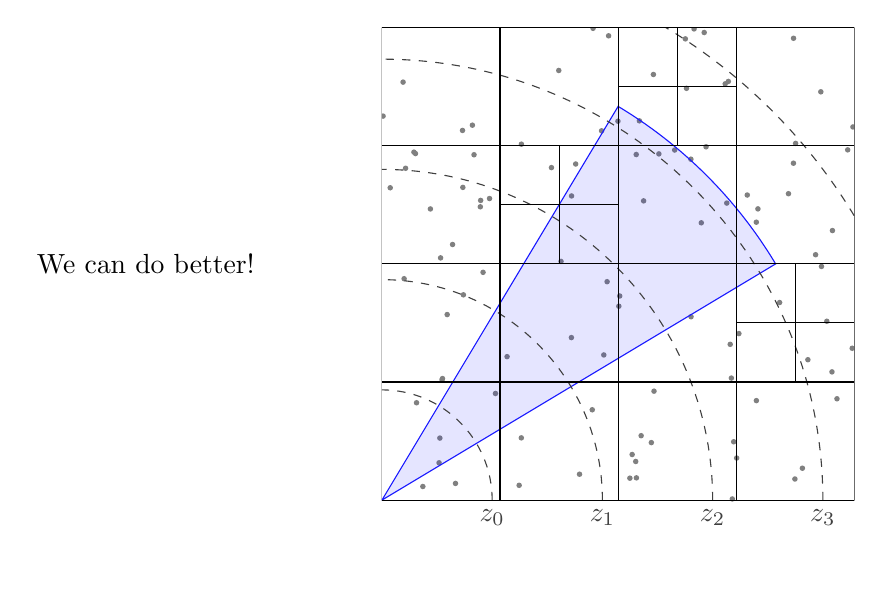
\begin{tikzpicture}
   % Text.
   \node at (-3,3) {We can do better!};
   % Border.
   \clip (0,-1) rectangle(6,6);
   \draw (0,0) rectangle(6,6);
   % Objects.
   \pgfmathsetseed{1187}
   \foreach \x in {1,...,100}
     \fill[black!50] ($ (0,0) + 6*(rnd,rnd) $) circle(1pt);
   % Cone.
   \filldraw[fill=blue,fill opacity=0.1,draw=blue!90] (0,0) -- (5,3) arc (30.96:59.04:5.83) -- cycle;
    % Redshift arcs.
    \begin{scope}
      \clip (0,-1) rectangle(6,6);
      \foreach \x/\z in {1.4/0, 2.8/1, 4.2/2, 5.6/3, 7/4}
        \draw[black!75,dashed] (\x,0) node[anchor=north]{$z_\z$} arc (0:90:\x);
    \end{scope}
   % Tree cells.
   \draw[step=1.5] (0,0) grid (6,6);
   \draw (2.25,3) -- (2.25,4.5); \draw (1.5,3.75) -- (3,3.75);
   \draw (5.25,1.5) -- (5.25,3); \draw (4.5,2.25) -- (6,2.25);
   \draw (3.75,4.5) -- (3.75,6); \draw (3,5.25) -- (4.5,5.25);
 \end{tikzpicture}
 \end{center}
\end{frame}

\begin{frame}[plain]
  \vspace{1cm}
  \begin{center}
 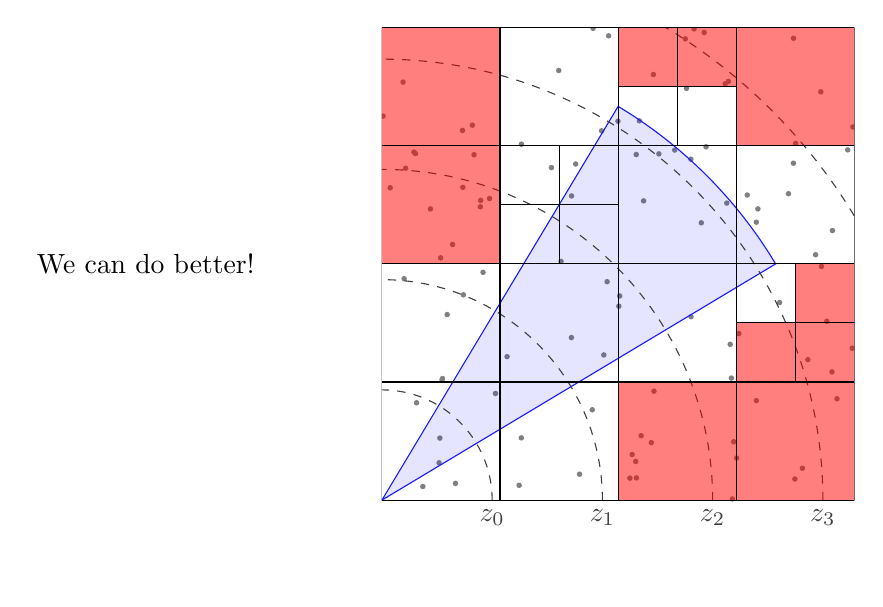
\begin{tikzpicture}
   % Text.
   \node at (-3,3) {We can do better!};
   % Border.
   \clip (0,-1) rectangle(6,6);
   \draw (0,0) rectangle(6,6);
   % Objects.
   \pgfmathsetseed{1187}
   \foreach \x in {1,...,100}
     \fill[black!50] ($ (0,0) + 6*(rnd,rnd) $) circle(1pt);
   % Cone.
   \filldraw[fill=blue,fill opacity=0.1,draw=blue!90] (0,0) -- (5,3) arc (30.96:59.04:5.83) -- cycle;
    % Redshift arcs.
    \begin{scope}
      \clip (0,-1) rectangle(6,6);
      \foreach \x/\z in {1.4/0, 2.8/1, 4.2/2, 5.6/3, 7/4}
        \draw[black!75,dashed] (\x,0) node[anchor=north]{$z_\z$} arc (0:90:\x);
    \end{scope}
   % Tree cells.
   \fill[fill=red,opacity=0.5] (3,0) rectangle (4.5,1.5);
   \fill[fill=red,opacity=0.5] (4.5,0) rectangle (6,1.5);
   \fill[fill=red,opacity=0.5] (0,3) rectangle (1.5,4.5);
   \fill[fill=red,opacity=0.5] (0,4.5) rectangle (1.5,6);
   \fill[fill=red,opacity=0.5] (4.5,4.5) rectangle (6,6);
   \fill[fill=red,opacity=0.5] (4.5,1.5) rectangle (5.25,2.25);
   \fill[fill=red,opacity=0.5] (5.25,1.5) rectangle (6,2.25);
   \fill[fill=red,opacity=0.5] (5.25,2.25) rectangle (6,3);
   \fill[fill=red,opacity=0.5] (3,5.25) rectangle (4.5,6);
   %% \fill[fill=red,opacity=0.5] (3.75,4.5) rectangle (4.5,5.25);
   \draw[step=1.5] (0,0) grid (6,6);
   \draw (2.25,3) -- (2.25,4.5); \draw (1.5,3.75) -- (3,3.75);
   \draw (5.25,1.5) -- (5.25,3); \draw (4.5,2.25) -- (6,2.25);
   \draw (3.75,4.5) -- (3.75,6); \draw (3,5.25) -- (4.5,5.25);
 \end{tikzpicture}
  \end{center}
\end{frame}

\begin{frame}[plain]
    \hspace{2cm}
    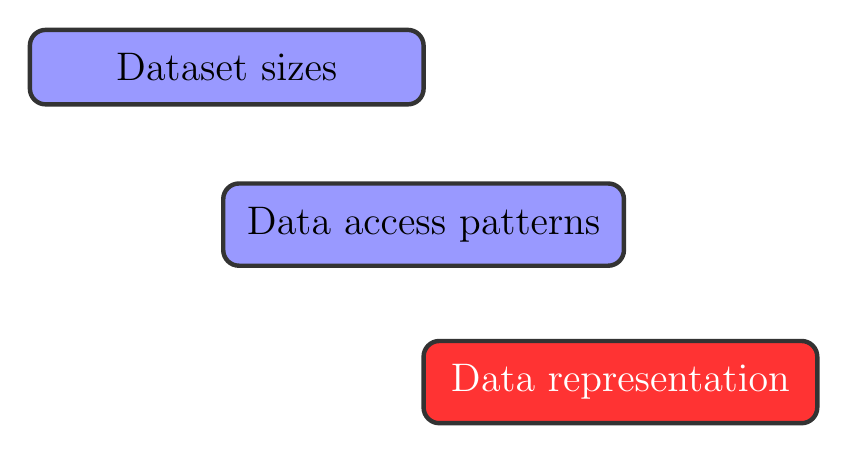
\begin{tikzpicture}[
        norm/.style={draw=black!80,rectangle,rounded corners=2mm,inner sep=3mm,fill=blue!40,ultra thick,minimum width=5cm},
        lit/.style={draw=black!80,rectangle,rounded corners=2mm,inner sep=3mm,fill=red!80,ultra thick,minimum width=5cm}
      ]
      \node[norm] at (0,0) {{\Large Dataset sizes}};
      \node[norm] at (2.5,-2) {{\Large Data access patterns}};
      \node[lit] at (5,-4) {{\Large \textcolor{white}{Data representation}}};
    \end{tikzpicture}
\end{frame}

\begin{frame}[plain]
  \begin{block}{Science Modules}
    \vspace{1cm}
    \hspace{2cm}
    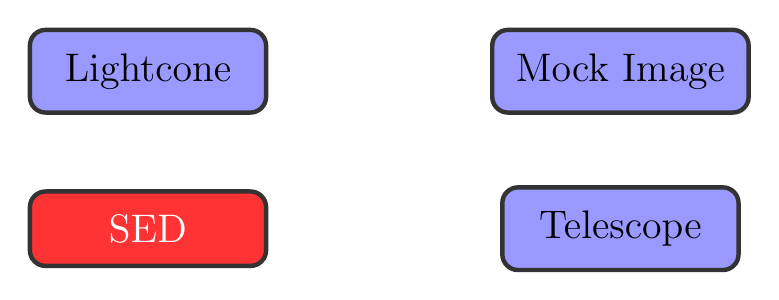
\begin{tikzpicture}[
        norm/.style={draw=black!80,rectangle,rounded corners=2mm,inner sep=3mm,fill=blue!40,ultra thick,minimum width=3cm},
        lit/.style={draw=black!80,rectangle,rounded corners=2mm,inner sep=3mm,fill=red!80,ultra thick,minimum width=3cm}
      ]
      \node[norm] at (0,0) {{\Large Lightcone}};
      \node[lit] at (0,-2) {{\Large \textcolor{white}{SED}}};
      \node[norm] at (6,0) {{\Large Mock Image}};
      \node[norm] at (6,-2) {{\Large Telescope}};
    \end{tikzpicture}
    \vspace{1cm}
  \end{block}
\end{frame}

\begin{frame}[plain]
 \begin{tikzpicture}[
     gal/.style={circle,draw},
     level 2/.style={sibling distance=10mm}
   ]
   \path[use as bounding box] (-2,-1.5) rectangle (8,6.5);
   % Merger trees.
   \node[gal] at (0,0) {I} [grow'=up]
     child {node {} edge from parent[dashed]};
   \node[gal] at (3,0) {A} [grow'=up]
     child {node[gal] {B}
       child {node[gal] {F}
         child {node[gal] {G}}
         child {node[gal] {H}}
       }
     }
     child {node[gal] {C}
       child {node[gal] {D}}
       child {node[gal] {E}}
     };
   \node[gal] at (6,0) {J} [grow'=up]
     child {node {} edge from parent[dashed]};
 \end{tikzpicture}
\end{frame}

\begin{frame}[plain]
 \begin{tikzpicture}[
     gal/.style={circle,draw},
     level 2/.style={sibling distance=10mm}
   ]
   \path[use as bounding box] (-2,-1.5) rectangle (8,6.5);
   % Merger trees.
   \node[gal] at (0,0) {I} [grow'=up]
     child {node {} edge from parent[dashed]};
   \node[gal] at (3,0) {A} [grow'=up]
     child {node[gal] {B}
       child {node[gal] {F}
         child {node[gal] {G}}
         child {node[gal] {H}}
       }
     }
     child {node[gal] {C}
       child {node[gal] {D}}
       child {node[gal] {E}}
     };
   \node[gal] at (6,0) {J} [grow'=up]
     child {node {} edge from parent[dashed]};
   % Pointers.
   \draw[-triangle 90] (5,5.5) node[anchor=west] {earliest galaxies} .. controls(2.25,5.5)and(2.25,5.5) .. (2.25,5);
 \end{tikzpicture}
\end{frame}

\begin{frame}[plain]
 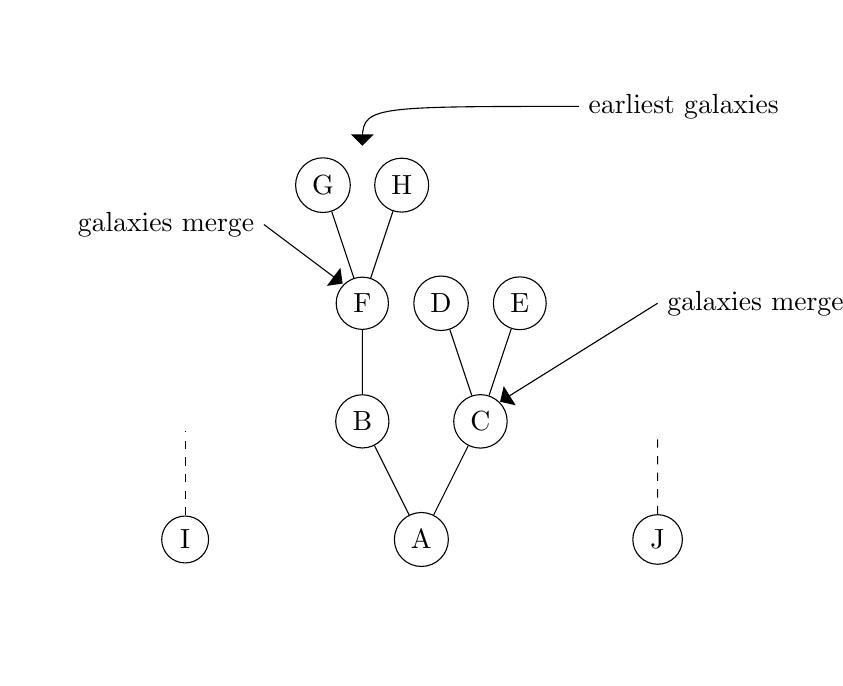
\begin{tikzpicture}[
     gal/.style={circle,draw},
     level 2/.style={sibling distance=10mm}
   ]
   \path[use as bounding box] (-2,-1.5) rectangle (8,6.5);
   % Merger trees.
   \node[gal] at (0,0) {I} [grow'=up]
     child {node {} edge from parent[dashed]};
   \node[gal] at (3,0) {A} [grow'=up]
     child {node[gal] {B}
       child {node[gal] {F}
         child {node[gal] {G}}
         child {node[gal] {H}}
       }
     }
     child {node[gal] {C}
       child {node[gal] {D}}
       child {node[gal] {E}}
     };
   \node[gal] at (6,0) {J} [grow'=up]
     child {node {} edge from parent[dashed]};
   % Pointers.
   \draw[-triangle 90] (5,5.5) node[anchor=west] {earliest galaxies} .. controls(2.25,5.5)and(2.25,5.5) .. (2.25,5);
   \draw[-triangle 90] (1,4) node[anchor=east] {galaxies merge} -- (2,3.25);
   \draw[-triangle 90] (6,3) node[anchor=west] {galaxies merge} -- (4,1.75);
 \end{tikzpicture}
\end{frame}

\begin{frame}[plain]
 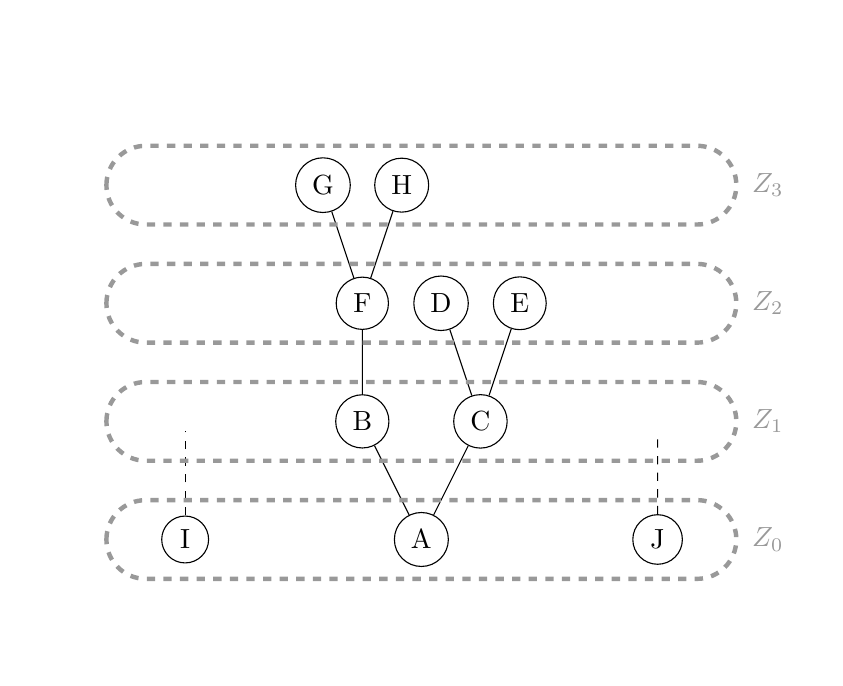
\begin{tikzpicture}[
     gal/.style={circle,draw},
     level 2/.style={sibling distance=10mm}
   ]
   \path[use as bounding box] (-2,-1.5) rectangle (8,6.5);
   % Merger trees.
   \node[gal] at (0,0) {I} [grow'=up]
     child {node {} edge from parent[dashed]};
   \node[gal] at (3,0) {A} [grow'=up]
     child {node[gal] {B}
       child {node[gal] {F}
         child {node[gal] {G}}
         child {node[gal] {H}}
       }
     }
     child {node[gal] {C}
       child {node[gal] {D}}
       child {node[gal] {E}}
     };
   \node[gal] at (6,0) {J} [grow'=up]
     child {node {} edge from parent[dashed]};
   % Snapshots.
   \draw[ultra thick,black!40,dashed,rounded corners=5mm] (-1,-0.5) rectangle (7,0.5) node[black!40] at (7.4,0) {$Z_0$};
   \draw[ultra thick,black!40,dashed,rounded corners=5mm] (-1,1) rectangle (7,2) node[black!40] at (7.4,1.5) {$Z_1$};
   \draw[ultra thick,black!40,dashed,rounded corners=5mm] (-1,2.5) rectangle (7,3.5) node[black!40] at (7.4,3) {$Z_2$};
   \draw[ultra thick,black!40,dashed,rounded corners=5mm] (-1,4) rectangle (7,5) node[black!40] at (7.4,4.5) {$Z_3$};
 \end{tikzpicture}
\end{frame}

\begin{frame}[plain]
 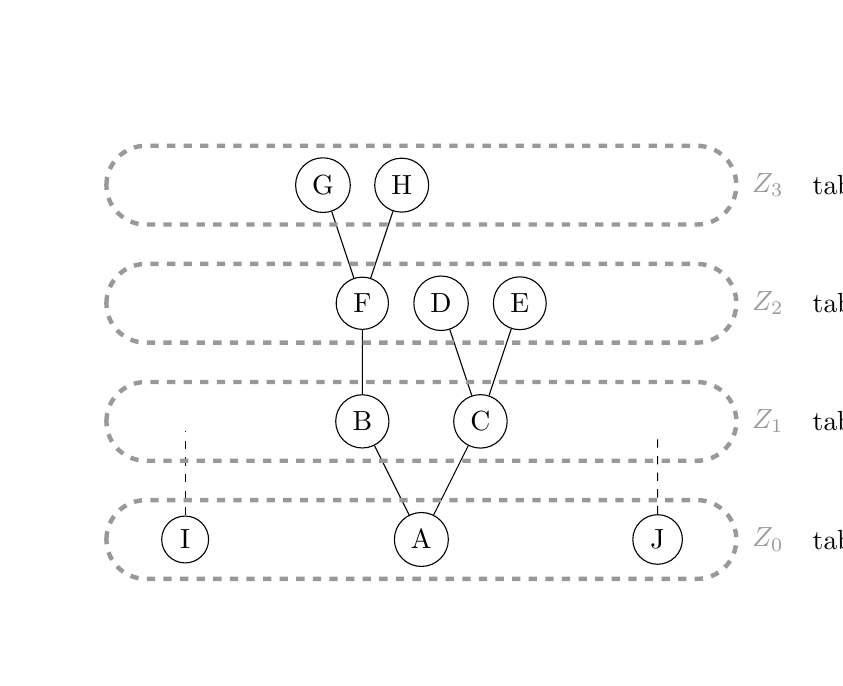
\begin{tikzpicture}[
     gal/.style={circle,draw},
     level 2/.style={sibling distance=10mm}
   ]
   \path[use as bounding box] (-2,-1.5) rectangle (8,6.5);
   % Merger trees.
   \node[gal] at (0,0) {I} [grow'=up]
     child {node {} edge from parent[dashed]};
   \node[gal] at (3,0) {A} [grow'=up]
     child {node[gal] {B}
       child {node[gal] {F}
         child {node[gal] {G}}
         child {node[gal] {H}}
       }
     }
     child {node[gal] {C}
       child {node[gal] {D}}
       child {node[gal] {E}}
     };
   \node[gal] at (6,0) {J} [grow'=up]
     child {node {} edge from parent[dashed]};
   % Snapshots.
   \draw[ultra thick,black!40,dashed,rounded corners=5mm] (-1,-0.5) rectangle (7,0.5) node[black!40] at (7.4,0) {$Z_0$} node[black] at (8.5,0) {table\_0};
   \draw[ultra thick,black!40,dashed,rounded corners=5mm] (-1,1) rectangle (7,2) node[black!40] at (7.4,1.5) {$Z_1$} node[black] at (8.5,1.5) {table\_1};
   \draw[ultra thick,black!40,dashed,rounded corners=5mm] (-1,2.5) rectangle (7,3.5) node[black!40] at (7.4,3) {$Z_2$} node[black] at (8.5,3) {table\_2};
   \draw[ultra thick,black!40,dashed,rounded corners=5mm] (-1,4) rectangle (7,5) node[black!40] at (7.4,4.5) {$Z_3$} node[black] at (8.5,4.5) {table\_3};
 \end{tikzpicture}
\end{frame}

\begin{frame}[plain]
 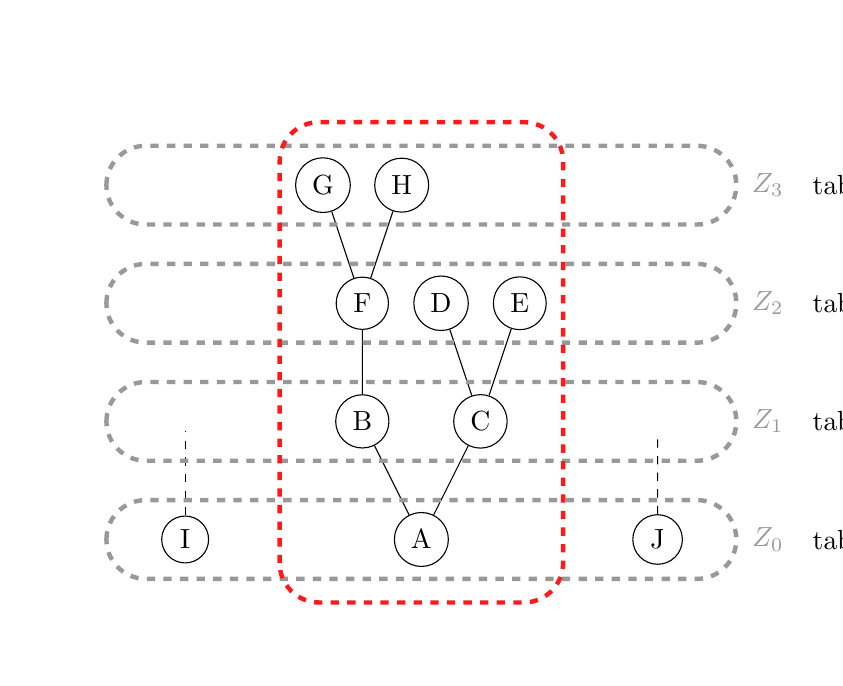
\begin{tikzpicture}[
     gal/.style={circle,draw},
     level 2/.style={sibling distance=10mm}
   ]
   \path[use as bounding box] (-2,-1.5) rectangle (8,6.5);
   % Merger trees.
   \node[gal] at (0,0) {I} [grow'=up]
     child {node {} edge from parent[dashed]};
   \node[gal] at (3,0) {A} [grow'=up]
     child {node[gal] {B}
       child {node[gal] {F}
         child {node[gal] {G}}
         child {node[gal] {H}}
       }
     }
     child {node[gal] {C}
       child {node[gal] {D}}
       child {node[gal] {E}}
     };
   \node[gal] at (6,0) {J} [grow'=up]
     child {node {} edge from parent[dashed]};
   % Snapshots.
   \draw[ultra thick,black!40,dashed,rounded corners=5mm] (-1,-0.5) rectangle (7,0.5) node[black!40] at (7.4,0) {$Z_0$} node[black] at (8.5,0) {table\_0};
   \draw[ultra thick,black!40,dashed,rounded corners=5mm] (-1,1) rectangle (7,2) node[black!40] at (7.4,1.5) {$Z_1$} node[black] at (8.5,1.5) {table\_1};
   \draw[ultra thick,black!40,dashed,rounded corners=5mm] (-1,2.5) rectangle (7,3.5) node[black!40] at (7.4,3) {$Z_2$} node[black] at (8.5,3) {table\_2};
   \draw[ultra thick,black!40,dashed,rounded corners=5mm] (-1,4) rectangle (7,5) node[black!40] at (7.4,4.5) {$Z_3$} node[black] at (8.5,4.5) {table\_3};
   % Forest.
   \draw[ultra thick,red!90,dashed,rounded corners=5mm] (1.2,-0.8) rectangle (4.8,5.3);
 \end{tikzpicture}
\end{frame}

\begin{frame}[plain]
 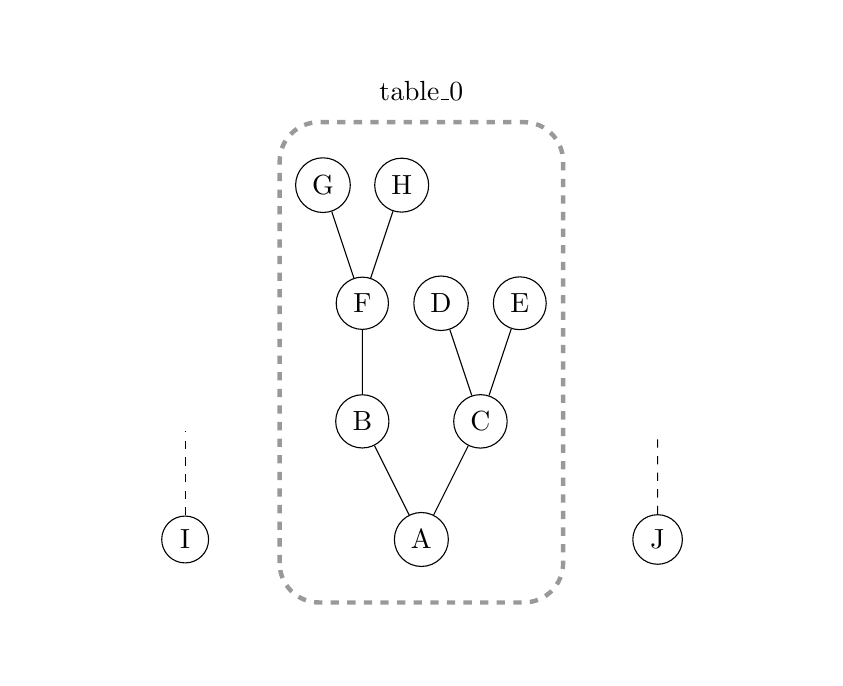
\begin{tikzpicture}[
     gal/.style={circle,draw},
     level 2/.style={sibling distance=10mm}
   ]
   \path[use as bounding box] (-2,-1.5) rectangle (8,6.5);
   % Merger trees.
   \node[gal] at (0,0) {I} [grow'=up]
     child {node {} edge from parent[dashed]};
   \node[gal] at (3,0) {A} [grow'=up]
     child {node[gal] {B}
       child {node[gal] {F}
         child {node[gal] {G}}
         child {node[gal] {H}}
       }
     }
     child {node[gal] {C}
       child {node[gal] {D}}
       child {node[gal] {E}}
     };
   \node[gal] at (6,0) {J} [grow'=up]
     child {node {} edge from parent[dashed]};
   % Forest.
   \draw[ultra thick,black!40,dashed,rounded corners=5mm] (1.2,-0.8) rectangle (4.8,5.3) node[black] at (3,5.7) {table\_0};
 \end{tikzpicture}
\end{frame}

%%
%% Rebinning.
%%

%% \begin{frame}[plain]
%%  \begin{tikzpicture}[
%%      gal/.style={circle,draw},
%%      main/.style={circle,draw,fill=red!80},
%%      lit/.style={circle,draw,fill=blue!40},
%%      level 2/.style={sibling distance=10mm}
%%    ]
%%    % Bounds.
%%    \path[use as bounding box] (-5,0) rectangle (5,6.5);
%%    % Text.
%%    \node at (-3.5,3) {Wrong timescale!};
%%    % Merger tree
%%    \node[gal] {A} [grow'=up]
%%      child {node[gal] {B}
%%        child {node[gal] {F}
%%          child {node[gal] {G}}
%%          child {node[gal] {H}}
%%        }
%%      }
%%      child {node[gal] {C}
%%        child {node[gal] {D}}
%%        child {node[gal] {E}}
%%      };
%%    % Snapshots.
%%    \draw (2.65,-0.05) -- (2.65,4.55);
%%    \foreach \y/\z in {-0.05/0, 1.55/1, 3.05/2, 4.55/3}
%%      \draw (2.6,\y) -- (2.7,\y) node[anchor=west] {$Z_\z$};
%%  \end{tikzpicture}
%% \end{frame}

%% \begin{frame}[plain]
%%  \begin{tikzpicture}[
%%      gal/.style={circle,draw},
%%      main/.style={circle,draw,fill=red!80},
%%      lit/.style={circle,draw,fill=blue!40},
%%      level 2/.style={sibling distance=10mm}
%%    ]
%%    % Bounds.
%%    \path[use as bounding box] (-5,0) rectangle (5,6.5);
%%    % Merger tree
%%    \node[main] {\textcolor{white}{A}} [grow'=up]
%%      child {node[lit] {B}
%%        child {node[lit] {F}
%%          child {node[lit] {G}}
%%          child {node[lit] {H}}
%%        }
%%      }
%%      child {node[lit] {C}
%%        child {node[lit] {D}}
%%        child {node[lit] {E}}
%%      };
%%    % Snapshots.
%%    \draw (2.65,-0.05) -- (2.65,4.55);
%%    \foreach \y/\z in {-0.05/0, 1.55/1, 3.05/2, 4.55/3}
%%      \draw (2.6,\y) -- (2.7,\y) node[anchor=west] {$Z_\z$};
%%    % Rebinning.
%%    \draw (4.05,-0.05) -- (4.05,6);
%%    \foreach \y/\z in {-0.05/0, 1/1, 3/2, 6/3}
%%      \draw (4,\y) -- (4.1,\y) node[anchor=west] {$\bar{Z}_\z$};
%%  \end{tikzpicture}
%% \end{frame}

%% \begin{frame}[plain]
%%  \begin{tikzpicture}[
%%      gal/.style={circle,draw},
%%      main/.style={circle,draw,fill=red!80},
%%      lit/.style={circle,draw,fill=blue!40},
%%      level 2/.style={sibling distance=10mm}
%%    ]
%%    % Bounds.
%%    \path[use as bounding box] (-5,0) rectangle (5,6.5);
%%    % Merger tree
%%    \node[gal] {A} [grow'=up]
%%      child {node[main] {\textcolor{white}{B}}
%%        child {node[lit] {F}
%%          child {node[lit] {G}}
%%          child {node[lit] {H}}
%%        }
%%      }
%%      child {node[gal] {C}
%%        child {node[gal] {D}}
%%        child {node[gal] {E}}
%%      };
%%    % Snapshots.
%%    \draw (2.65,-0.05) -- (2.65,4.55);
%%    \foreach \y/\z in {-0.05/0, 1.55/1, 3.05/2, 4.55/3}
%%      \draw (2.6,\y) -- (2.7,\y) node[anchor=west] {$Z_\z$};
%%    % Rebinning.
%%    \draw (4.05,1.55) -- (4.05,4.6);
%%    \draw[dashed] (4.05,4.6) -- (4.05,6);
%%    \foreach \y/\z in {1.55/0, 2.6/1, 4.6/2}
%%      \draw (4,\y) -- (4.1,\y) node[anchor=west] {$\bar{Z}_\z$};
%%  \end{tikzpicture}
%% \end{frame}

\begin{frame}[plain]
  \Large
  \begin{columns}[c]
    \column{7cm}
    \begin{exampleblock}{}
      Database is looking good...
    \end{exampleblock}
    \column{4cm}
  \end{columns}
  \vspace{2cm}
  \begin{columns}[c]
    \column{3cm}
    \column{8cm}
    \begin{exampleblock}{}
      ... what about large computation?
    \end{exampleblock}
  \end{columns}
\end{frame}

\begin{frame}[plain]
  \Large
  \begin{columns}[c]
    \column{7cm}
    \begin{exampleblock}{}
      $\approx$ 2.5 billion galaxies in Bolshoi dataset,
      how many to process, on average, per request?
    \end{exampleblock}
    \column{4cm}
  \end{columns}
  \vspace{2cm}
  \begin{columns}[c]
    \column{3cm}
    \column{8cm}
    \begin{exampleblock}{}
      We will need to parallelise computation.
    \end{exampleblock}
  \end{columns}
\end{frame}

\begin{frame}[plain]
  \begin{block}{Science Modules}
    \vspace{1cm}
    \hspace{2cm}
    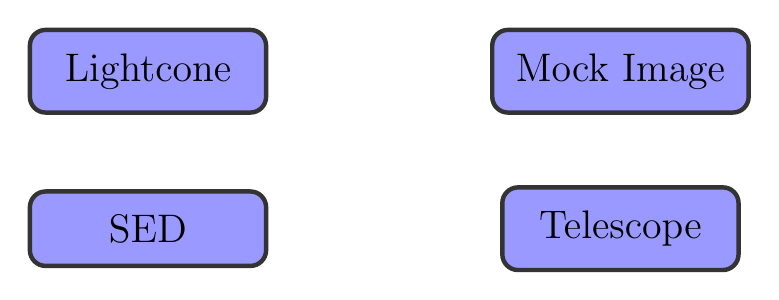
\begin{tikzpicture}[
        norm/.style={draw=black!80,rectangle,rounded corners=2mm,inner sep=3mm,fill=blue!40,ultra thick,minimum width=3cm}
      ]
      \node[norm] (lc) at (0,0) {{\Large Lightcone}};
      \node[norm] (sed) at (0,-2) {{\Large SED}};
      \node[norm] (mi) at (6,0) {{\Large Mock Image}};
      \node[norm] (te) at (6,-2) {{\Large Telescope}};
    \end{tikzpicture}
    \vspace{1cm}
  \end{block}
\end{frame}

\begin{frame}[plain]
  \begin{block}{Science Modules}
    \vspace{1cm}
    \hspace{2cm}
    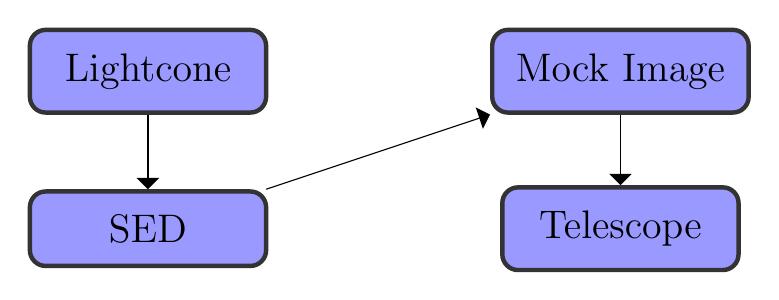
\begin{tikzpicture}[
        norm/.style={draw=black!80,rectangle,rounded corners=2mm,inner sep=3mm,fill=blue!40,ultra thick,minimum width=3cm}
      ]
      \node[norm] (lc) at (0,0) {{\Large Lightcone}};
      \node[norm] (sed) at (0,-2) {{\Large SED}};
      \node[norm] (mi) at (6,0) {{\Large Mock Image}};
      \node[norm] (te) at (6,-2) {{\Large Telescope}};
      % Connections.
      \draw[-triangle 90] (lc) -- (sed);
      \draw[-triangle 90] (sed) -- (mi);
      \draw[-triangle 90] (mi) -- (te);
    \end{tikzpicture}
    \vspace{1cm}
  \end{block}
\end{frame}

\begin{frame}[plain]
  \begin{center}
  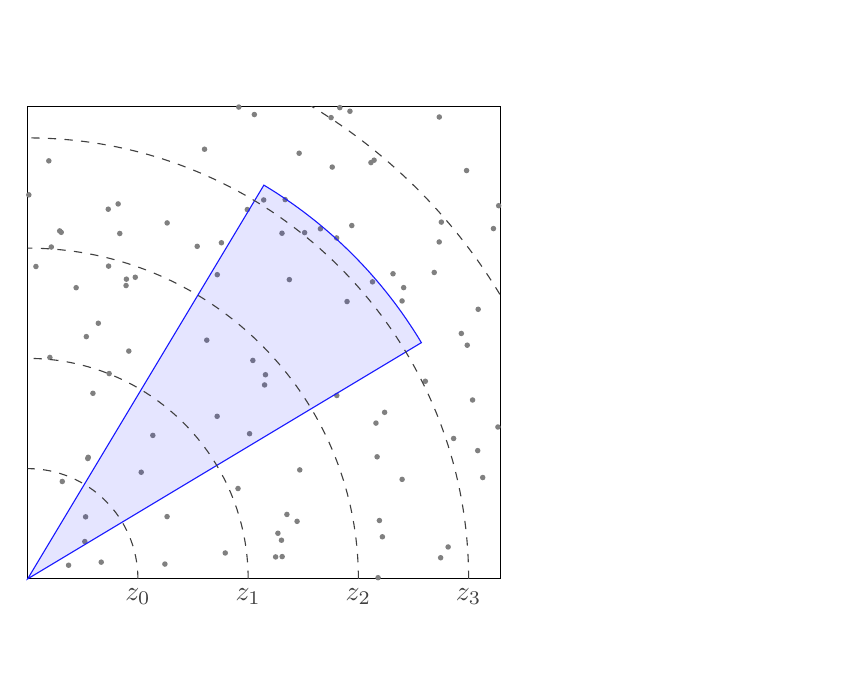
\begin{tikzpicture}
    \path[use as bounding box] (0,-1) rectangle (10,7);
    % Border.
    \draw (0,0) rectangle (6,6);
    % Objects.
    \pgfmathsetseed{1187}
    \foreach \x in {1,...,100}
    \fill[black!50] ($ (0,0) + 6*(rnd,rnd) $) circle(1pt);
    % Cone.
    \filldraw[fill=blue,fill opacity=0.1,draw=blue!90] (0,0) -- (5,3) arc (30.96:59.04:5.83) -- cycle;
    % Redshift arcs.
    \begin{scope}
      \clip (0,-1) rectangle(6,6);
      \foreach \x/\z in {1.4/0, 2.8/1, 4.2/2, 5.6/3, 7/4}
        \draw[black!75,dashed] (\x,0) node[anchor=north]{$z_\z$} arc (0:90:\x);
    \end{scope}
  \end{tikzpicture}
  \end{center}
\end{frame}

\begin{frame}[plain]
  \begin{center}
  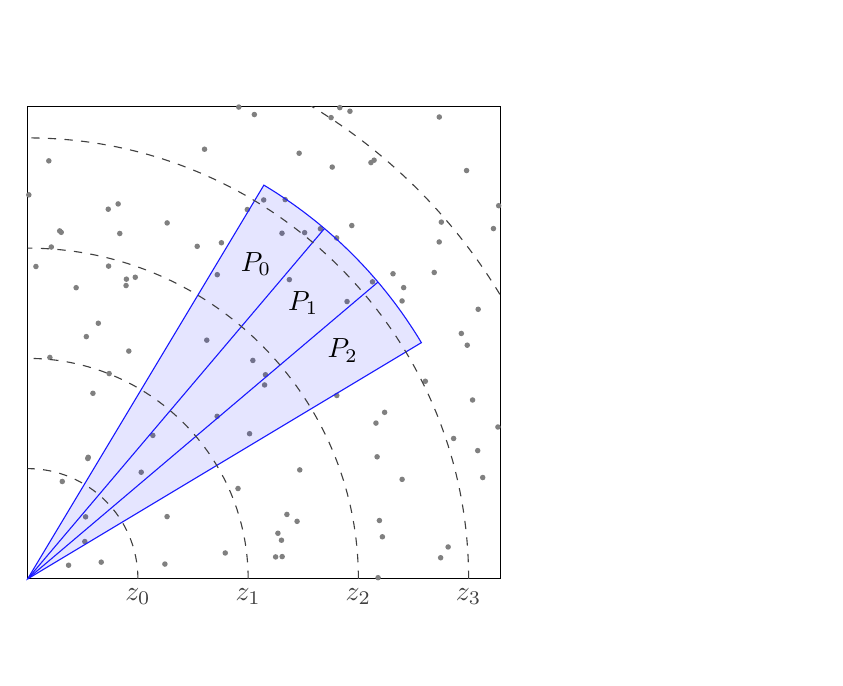
\begin{tikzpicture}
    \path[use as bounding box] (0,-1) rectangle (10,7);
    % Border.
    \draw (0,0) rectangle (6,6);
    % Objects.
    \pgfmathsetseed{1187}
    \foreach \x in {1,...,100}
    \fill[black!50] ($ (0,0) + 6*(rnd,rnd) $) circle(1pt);
    % Cone.
    \filldraw[fill=blue,fill opacity=0.1,draw=blue!90] (0,0) -- (5,3) arc (30.96:59.04:5.83) -- cycle;
   \draw[blue!90] (0,0) -- (4.45,3.77);
   \draw[blue!90] (0,0) -- (3.77,4.45);
   \draw (2.9,4) node{$P_0$};
   \draw (3.5,3.5) node{$P_1$};
   \draw (4,2.9) node{$P_2$};
    % Redshift arcs.
    \begin{scope}
      \clip (0,-1) rectangle(6,6);
      \foreach \x/\z in {1.4/0, 2.8/1, 4.2/2, 5.6/3, 7/4}
        \draw[black!75,dashed] (\x,0) node[anchor=north]{$z_\z$} arc (0:90:\x);
    \end{scope}
  \end{tikzpicture}
  \end{center}
\end{frame}

\begin{frame}[plain]
  \begin{center}
  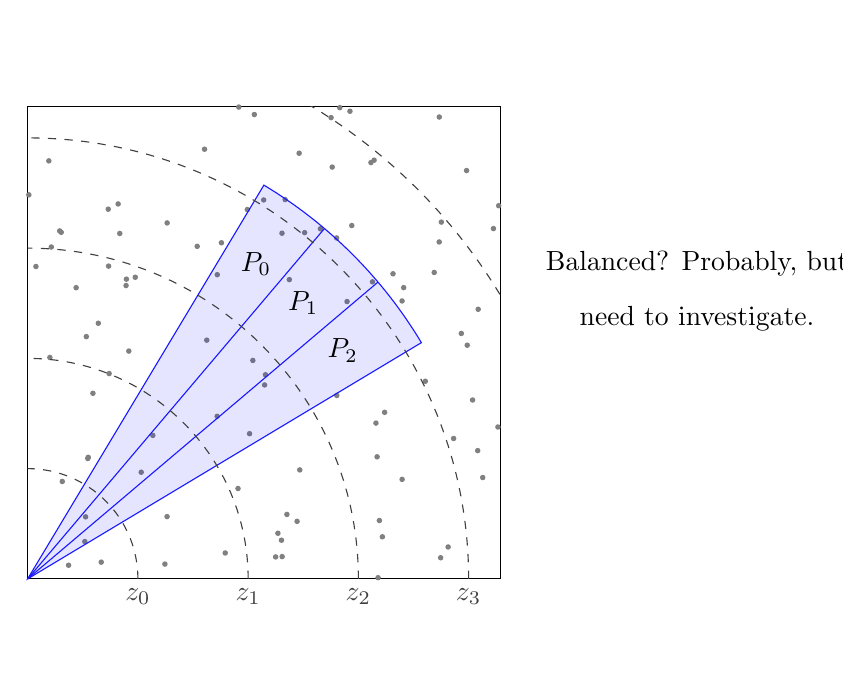
\begin{tikzpicture}
    \path[use as bounding box] (0,-1) rectangle (10,7);
    % Border.
    \draw (0,0) rectangle (6,6);
    % Objects.
    \pgfmathsetseed{1187}
    \foreach \x in {1,...,100}
    \fill[black!50] ($ (0,0) + 6*(rnd,rnd) $) circle(1pt);
    % Cone.
    \filldraw[fill=blue,fill opacity=0.1,draw=blue!90] (0,0) -- (5,3) arc (30.96:59.04:5.83) -- cycle;
   \draw[blue!90] (0,0) -- (4.45,3.77);
   \draw[blue!90] (0,0) -- (3.77,4.45);
   \draw (2.9,4) node{$P_0$};
   \draw (3.5,3.5) node{$P_1$};
   \draw (4,2.9) node{$P_2$};
    % Redshift arcs.
    \begin{scope}
      \clip (0,-1) rectangle(6,6);
      \foreach \x/\z in {1.4/0, 2.8/1, 4.2/2, 5.6/3, 7/4}
        \draw[black!75,dashed] (\x,0) node[anchor=north]{$z_\z$} arc (0:90:\x);
    \end{scope}
    % Text.
    \node at (8.5,4) {Balanced? Probably, but};
    \node at (8.5,3.3) {need to investigate.};
  \end{tikzpicture}
  \end{center}
\end{frame}

\begin{frame}[plain]
  \Large
  \begin{columns}[c]
    \column{7cm}
    \begin{exampleblock}{}
      We will also utilise GPUs (eventually).
    \end{exampleblock}
    \column{4cm}
  \end{columns}
  \vspace{2cm}
  \begin{columns}[c]
    \column{3cm}
    \column{8cm}
    \begin{block}{Algorithms}
      \begin{itemize}
        \item Cubic spline interpolation.
        \item Fourth order Gaussian integration.
        \item Both easily accelerated by GPUs.
      \end{itemize}
    \end{block}
  \end{columns}
\end{frame}


%% \begin{frame}[plain]
%%   \insertpicture{test.png}
%% \end{frame}

%% \begin{frame}[plain]
%%  $A$ time bins \\
%%  $M$ galaxies in merger tree branch \\
%%  $N$ root galaxies in lightcone \\
%%  $AMN$
%%  for every root galaxy, $g$,
%% \end{frame}

%% \begin{frame}[plain]
%%  \begin{block}{Triple Loop}
%%    \[ S_i = \sum_j^n \sum_k^a \sum_k^m ssp_{ijk} \]
%%  \end{block}
%% \end{frame}

%% \begin{frame}[plain]
%%  \begin{block}{Convolution}
%%    \begin{eqnarray*}
%%      I & = & f_\lambda*s_\lambda \\
%%        & = & \int_{\nu_l}^{\nu_U}f_{\nu}s_{\nu}d\nu \\
%%        & \approx & \sum_i^{n_{\nu}}f_is_i
%%    \end{eqnarray*}
%%  \end{block}
%% \end{frame}

%% \begin{frame}[plain]
%%  \begin{block}{Complexity}
%%    \begin{eqnarray*}
%%      I & = & f_\lambda*s_\lambda \\
%%        & = & \int_{\nu_l}^{\nu_U}f_{\nu}s_{\nu}d\nu \\
%%        & \approx & \sum_i^{n_{\nu}}f_is_i
%%    \end{eqnarray*}
%%  \end{block}
%% \end{frame}

%% \begin{frame}{Using GPU Hardware}
%%  \begin{block}{Methods}
%%    \begin{itemize}
%%      \item Cubic spline interpolation.
%%      \item Fourth order gaussian quadrature integration.
%%      \item Both easily implemented on GPU hardware.
%%    \end{itemize}
%%  \end{block}
%% \end{frame}

%% \begin{frame}{Cubic Spline}
%%  \begin{eqnarray*}
%%      f(x) & = & (1 - t)y_1 + ty_2 + t(1 - t)(a(1 - t) + bt) \\
%%      t & = & \frac{x - x_1}{x_2 - x_1} \\
%%      a & = & k_1(x_2 - x_1) - (y_2 - y_1) \\
%%      b & = & -k_2(x_2 - x_1) + (y_2 + y_1)
%%  \end{eqnarray*}
%%  \begin{block}{Advantages}
%%    \begin{itemize}
%%      \item Third order piecewise polynomials.
%%      \item Smooth function.
%%      \item Smooth derivatives.
%%      \item Immune to oscillatory problems of non-piecewise methods.
%%    \end{itemize}
%%  \end{block}
%% \end{frame}

%% \begin{frame}{Using GPU Hardware}
%%  \begin{block}{Fourth Order Gaussian}
%%    \begin{itemize}
%%      \item Integrates third order polyomial exactly.
%%      \item Simple implementation.
%%      \item Very efficient.
%%    \end{itemize}
%%  \end{block}
%% \end{frame}

%% \begin{frame}{Using GPU Hardware}
%% \end{frame}


%% \begin{frame}{Ordering}
%%  \begin{tikzpicture}[
%%      gal/.style={circle,draw},
%%      level 2/.style={sibling distance=10mm}
%%    ]
%%    % Merger trees.
%%    \node[gal] at (3,0) {A} [grow'=up]
%%      child {node[gal] {B}
%%        child {node[gal] {F}
%%          child {node[gal] {G}}
%%          child {node[gal] {H}}
%%        }
%%      }
%%      child {node[gal] {C}
%%        child {node[gal] {D}}
%%        child {node[gal] {E}}
%%      };
%%  \end{tikzpicture}
%% \end{frame}

%% \begin{frame}{Ordering}
%%  \begin{tikzpicture}[
%%      gal/.style={circle,draw},
%%      level 2/.style={sibling distance=10mm}
%%    ]
%%    % Merger trees.
%%    \node[gal] at (3,0) {0} [grow'=up]
%%      child {node[gal] {1}
%%        child {node[gal] {2}
%%          child {node[gal] {3}}
%%          child {node[gal] {4}}
%%        }
%%      }
%%      child {node[gal] {5}
%%        child {node[gal] {6}}
%%        child {node[gal] {7}}
%%      };
%%  \end{tikzpicture}
%% \end{frame}

%% \begin{frame}{Ordering}
%%  \begin{tikzpicture}[
%%      gal/.style={circle,draw},
%%      level 2/.style={sibling distance=10mm}
%%    ]
%%    % Merger trees.
%%    \node[gal] at (3,0) {0} [grow'=up]
%%      child {node[gal] {1}
%%        child {node[gal] {2}
%%          child {node[gal] {3}}
%%          child {node[gal] {4}}
%%        }
%%      }
%%      child {node[gal] {5}
%%        child {node[gal] {6}}
%%        child {node[gal] {7}}
%%      };
%%    % Flattened array.
%%    \foreach \x in {5, 6, 7, 8, 9, 10, 11, 12, 13}
%%      \draw (\x,1) -- (\x,2);
%%    \draw (5,1) -- (13,1);
%%    \draw (5,2) -- (13,2);
%%    \foreach \x/\n in {5.5/0, 6.5/1, 7.5/2, 8.5/3, 9.5/4, 10.5/5, 11.5/6, 12.5/7}
%%      \node at (\x,1.5) {\n};
%%  \end{tikzpicture}
%% \end{frame}

%% \begin{frame}{Ordering}
%%  \begin{tikzpicture}[
%%      gal/.style={circle,draw},
%%      main/.style={circle,draw,fill=red!80},
%%      lit/.style={circle,draw,fill=blue!40},
%%      level 2/.style={sibling distance=10mm}
%%    ]
%%    % Merger trees.
%%    \node[gal] at (3,0) {0} [grow'=up]
%%      child {node[gal] {\textcolor{white}{1}}
%%        child {node[main] {\textcolor{white}{2}}
%%          child {node[lit] {3}}
%%          child {node[lit] {4}}
%%        }
%%      }
%%      child {node[gal] {5}
%%        child {node[gal] {6}}
%%        child {node[gal] {7}}
%%      };
%%    % Flattened array.
%%    \node at (5.5,1.5) {0};
%%    \node at (6.5,1.5) {1};
%%    \node[rectangle,minimum size=10mm,fill=red!80] at (7.5,1.5) {\textcolor{white}{2}};
%%    \node[rectangle,minimum size=10mm,fill=blue!40] at (8.5,1.5) {3};
%%    \node[rectangle,minimum size=10mm,fill=blue!40] at (9.5,1.5) {4};
%%    \node at (10.5,1.5) {5};
%%    \node at (11.5,1.5) {6};
%%    \node at (12.5,1.5) {7};
%%    \foreach \x in {5, 6, 7, 8, 9, 10, 11, 12, 13}
%%      \draw (\x,1) -- (\x,2);
%%    \draw (5,1) -- (13,1);
%%    \draw (5,2) -- (13,2);
%%  \end{tikzpicture}
%% \end{frame}

%% \begin{frame}{Ordering}
%%  \begin{tikzpicture}[
%%      gal/.style={circle,draw},
%%      main/.style={circle,draw,fill=red!80},
%%      lit/.style={circle,draw,fill=blue!40},
%%      level 2/.style={sibling distance=10mm}
%%    ]
%%    % Merger trees.
%%    \node[gal] at (3,0) {0} [grow'=up]
%%      child {node[main] {\textcolor{white}{1}}
%%        child {node[lit] {2}
%%          child {node[lit] {3}}
%%          child {node[lit] {4}}
%%        }
%%      }
%%      child {node[gal] {5}
%%        child {node[gal] {6}}
%%        child {node[gal] {7}}
%%      };
%%    % Flattened array.
%%    \node at (5.5,1.5) {0};
%%    \node[rectangle,minimum size=10mm,fill=red!80] at (6.5,1.5) {\textcolor{white}{1}};
%%    \node[rectangle,minimum size=10mm,fill=blue!40] at (7.5,1.5) {2};
%%    \node[rectangle,minimum size=10mm,fill=blue!40] at (8.5,1.5) {3};
%%    \node[rectangle,minimum size=10mm,fill=blue!40] at (9.5,1.5) {4};
%%    \node at (10.5,1.5) {5};
%%    \node at (11.5,1.5) {6};
%%    \node at (12.5,1.5) {7};
%%    \foreach \x in {5, 6, 7, 8, 9, 10, 11, 12, 13}
%%      \draw (\x,1) -- (\x,2);
%%    \draw (5,1) -- (13,1);
%%    \draw (5,2) -- (13,2);
%%  \end{tikzpicture}
%% \end{frame}

%% \begin{frame}[plain]
%%  \begin{tikzpicture}[
%%      gal/.style={circle,draw},
%%      level 2/.style={sibling distance=10mm}
%%    ]
%%    % Merger tree
%%    \node[gal] {A} [grow'=up]
%%      child {node[gal] {B}
%%        child {node[gal] {F}
%%          child {node[gal] {G}}
%%          child {node[gal] {H}}
%%        }
%%      }
%%      child {node[gal] {C}
%%        child {node[gal] {D}}
%%        child {node[gal] {E}}
%%      };
%%    % Snapshots.
%%    \draw (2.65,-0.05) -- (2.65,4.55);
%%    \foreach \y/\z in {-0.05/0, 1.55/1, 3.05/2, 4.55/3}
%%      \draw (2.6,\y) -- (2.7,\y) node[anchor=west] {$Z_\z$};
%%  \end{tikzpicture}
%% \end{frame}

\end{document}
